% Created 2024-07-03 Mi 09:33
% Intended LaTeX compiler: pdflatex
\documentclass[11pt]{article}
\usepackage[utf8]{inputenc}
\usepackage[T1]{fontenc}
\usepackage{graphicx}
\usepackage{longtable}
\usepackage{wrapfig}
\usepackage{rotating}
\usepackage[normalem]{ulem}
\usepackage{amsmath}
\usepackage{amssymb}
\usepackage{capt-of}
\usepackage{hyperref}
\author{Yannik Bürkle, Marcus Herrmann, Dennis Reise}
\date{\textit{<2024-05-17 Fr>}}
\title{Projektarbeit Netzwerk Dokumentation}
\hypersetup{
 pdfauthor={Yannik Bürkle, Marcus Herrmann, Dennis Reise},
 pdftitle={Projektarbeit Netzwerk Dokumentation},
 pdfkeywords={},
 pdfsubject={},
 pdfcreator={Emacs 29.4 (Org mode 9.8)}, 
 pdflang={English}}
\begin{document}

\maketitle
\tableofcontents

\section{MAC-Adressen-Tabellen}
\label{sec:org6f036d5}
\subsection{SWSERVERROOM}
\label{sec:org0246152}
\begin{verbatim}
SWSERVERROOM#show mac-address-table
          Mac Address Table
-------------------------------------------

Vlan    Mac Address       Type        Ports
----    -----------       --------    -----

  10    0001.43b8.6c01    DYNAMIC     Gig0/2
  10    0001.64be.b617    DYNAMIC     Fa0/2
  10    0001.c963.aae3    DYNAMIC     Gig0/1
  10    0006.2a52.5372    DYNAMIC     Gig0/1
  10    0090.2b11.6254    DYNAMIC     Gig0/1
  10    00d0.bcbe.b68a    DYNAMIC     Fa0/22
  10    00e0.8f60.9dcd    DYNAMIC     Fa0/23
  10    00e0.f758.668e    DYNAMIC     Gig0/1
  20    0001.43b8.6c01    DYNAMIC     Gig0/2
  20    0001.43eb.baea    DYNAMIC     Fa0/23
  20    0001.97d4.3b62    DYNAMIC     Fa0/23
  20    0004.9a2a.0553    DYNAMIC     Fa0/23
  20    0007.ec9b.9670    DYNAMIC     Fa0/23
  20    0040.0b5a.7743    DYNAMIC     Fa0/23
  20    00e0.f7eb.7845    DYNAMIC     Fa0/23
  30    0001.43b8.6c01    DYNAMIC     Gig0/2
  40    0001.c946.8201    DYNAMIC     Fa0/1
  40    000b.be06.0a01    DYNAMIC     Fa0/24
  40    00d0.5831.aa01    DYNAMIC     Gig0/1
  40    00e0.a31a.5b56    DYNAMIC     Fa0/21
\end{verbatim}
\subsection{SWBUERO}
\label{sec:orge25d151}
\begin{verbatim}
SWBUERO#show mac-address-table
          Mac Address Table
-------------------------------------------

Vlan    Mac Address       Type        Ports
----    -----------       --------    -----

  10    0001.43b8.6c01    DYNAMIC     Gig0/1
  10    0001.64be.b617    DYNAMIC     Gig0/1
  10    0001.64e2.4119    DYNAMIC     Gig0/1
  10    0001.c963.aae3    DYNAMIC     Fa0/3
  10    0006.2a52.5372    DYNAMIC     Fa0/1
  10    0090.2b11.6254    DYNAMIC     Fa0/4
  10    00e0.8f60.9dcd    DYNAMIC     Gig0/1
  10    00e0.f758.668e    DYNAMIC     Fa0/2
  10    0001.6478.ac12    DYNAMIC     Gig0/1
  30    0001.64e2.4119    DYNAMIC     Gig0/1
  40    0001.64e2.4119    DYNAMIC     Gig0/1
  40    00d0.5831.aa01    DYNAMIC     Fa0/24
  40    00e0.a31a.5b56    DYNAMIC     Gig0/1
\end{verbatim}
\subsection{SWLABOR}
\label{sec:orga2b231c}
\begin{verbatim}
SWLABOR#show mac-address-table
          Mac Address Table
-------------------------------------------

Vlan    Mac Address       Type        Ports
----    -----------       --------    -----

  10    0001.43b8.6c01    DYNAMIC     Fa0/24
  10    0001.64be.b617    DYNAMIC     Fa0/24
  10    0001.64e2.4117    DYNAMIC     Fa0/24
  10    0001.c963.aae3    DYNAMIC     Fa0/24
  10    0006.2a52.5372    DYNAMIC     Fa0/24
  10    0090.2b11.6254    DYNAMIC     Fa0/24
  10    00e0.8f60.9dcd    DYNAMIC     Fa0/1
  10    00e0.f758.668e    DYNAMIC     Fa0/24
  20    0001.43b8.6c01    DYNAMIC     Fa0/24
  20    0001.43eb.baea    DYNAMIC     Fa0/11
  20    0001.64e2.4117    DYNAMIC     Fa0/24
  20    0001.97d4.3b62    DYNAMIC     Fa0/21
  20    0004.9a2a.0553    DYNAMIC     Fa0/10
  20    0007.ec9b.9670    DYNAMIC     Fa0/13
  20    0040.0b5a.7743    DYNAMIC     Fa0/20
  20    00e0.f7eb.7845    DYNAMIC     Fa0/12
\end{verbatim}
\subsection{SWMEETING}
\label{sec:orgdcb8961}
\begin{verbatim}
SWMEETING#sh mac-address-table
          Mac Address Table
-------------------------------------------

Vlan    Mac Address       Type        Ports
----    -----------       --------    -----

  10    0001.43b8.6c01    DYNAMIC     Fa0/24
  10    0001.64e2.4118    DYNAMIC     Fa0/24
  10    0001.c963.aae3    DYNAMIC     Fa0/24
  10    0090.2b11.6254    DYNAMIC     Fa0/24
  10    00e0.8f60.9dcd    DYNAMIC     Fa0/24
  10    0001.6478.ac12    DYNAMIC     Fa0/2
  10    0006.2a52.5372    DYNAMIC     Fa0/24
  30    0001.64e2.4118    DYNAMIC     Fa0/24
  40    0001.64e2.4118    DYNAMIC     Fa0/24
  40    000b.be06.0a01    DYNAMIC     Fa0/1
  40    00e0.a31a.5b56    DYNAMIC     Fa0/24
\end{verbatim}
\section{Routingtabelle RTR1}
\label{sec:orgefc943e}
\begin{verbatim}
RTR1#show ip route
Codes: L - local, C - connected, S - static, R - RIP, M - mobile, B - BGP
[output shortened]

Gateway of last resort is not set
 *   0.0.0.0/1 is subnetted, 1 subnets
C*      0.0.0.0/1 is directly connected, GigabitEthernet0/1
     45.0.0.0/32 is subnetted, 1 subnets
L       45.232.17.11/32 is directly connected, GigabitEthernet0/1
     172.19.0.0/16 is variably subnetted, 8 subnets, 2 masks
C       172.19.0.0/25 is directly connected, GigabitEthernet0/0.10
L       172.19.0.1/32 is directly connected, GigabitEthernet0/0.10
C       172.19.0.128/25 is directly connected, GigabitEthernet0/0.20
L       172.19.0.129/32 is directly connected, GigabitEthernet0/0.20
C       172.19.1.0/25 is directly connected, GigabitEthernet0/0.30
L       172.19.1.1/32 is directly connected, GigabitEthernet0/0.30
C       172.19.1.128/25 is directly connected, GigabitEthernet0/0.40
L       172.19.1.129/32 is directly connected, GigabitEthernet0/0.40

RTR1#show ipv6 route
IPv6 Routing Table - 15 entries
Codes: C - Connected, L - Local, S - Static, R - RIP, B - BGP
[output shortened]
C   2001:DB8:0:0:10::/80 [0/0]
     via GigabitEthernet0/0.10, directly connected
L   2001:DB8::10:0:0:1/128 [0/0]
     via GigabitEthernet0/0.10, receive
C   2001:DB8:0:0:20::/80 [0/0]
     via GigabitEthernet0/0.20, directly connected
L   2001:DB8::20:0:0:1/128 [0/0]
     via GigabitEthernet0/0.20, receive
C   2001:DB8:0:0:30::/80 [0/0]
     via GigabitEthernet0/0.30, directly connected
L   2001:DB8::30:0:0:1/128 [0/0]
     via GigabitEthernet0/0.30, receive
C   2001:DB8:0:10::/64 [0/0]
     via GigabitEthernet0/0.10, directly connected
L   2001:DB8:0:10::1/128 [0/0]
     via GigabitEthernet0/0.10, receive
C   2001:DB8:0:20::/64 [0/0]
     via GigabitEthernet0/0.20, directly connected
L   2001:DB8:0:20::1/128 [0/0]
     via GigabitEthernet0/0.20, receive
C   2001:DB8:0:30::/64 [0/0]
     via GigabitEthernet0/0.30, directly connected
L   2001:DB8:0:30::1/128 [0/0]
     via GigabitEthernet0/0.30, receive
C   2001:DB8:0:40::/64 [0/0]
     via GigabitEthernet0/0.40, directly connected
L   2001:DB8:0:40::1/128 [0/0]
     via GigabitEthernet0/0.40, receive
L   FF00::/8 [0/0]
     via Null0, receive
\end{verbatim}

Die Routingtabelle von RTR1 ist also sehr simpel. Alle Netze sind direkt verbunden über die verschiedenen Subinterfaces von GigabitEthernet0/0.
\section{Netze und ihre Eigenschaften}
\label{sec:orgfe04721}
\subsection{Firmennetz}
\label{sec:org27af5b4}
\begin{itemize}
\item VLAN ID: 10
\item CISCO VLAN Name: ``FIRMENNETZ''
\item IPv4-Bereich: 172.19.0.0/25
\item IPv4-Gateway: 172.19.0.1
\item IPv6-Bereich: 2001:db8:0:10::/64
\item IPv6-Gateway: fe80::1
\end{itemize}
\subsection{IoT-Netzwerk}
\label{sec:orgae17260}
\begin{itemize}
\item VLAN ID: 20
\item CISCO VLAN Name: ``IoT-Netz''
\item IPv4-Bereich: 172.19.0.128/25
\item IPv4-Gateway: 172.19.0.129
\item IPv6-Bereich: 2001:db8:0:20::/64
\item IPv6-Gateway: fe80::1
\end{itemize}
\subsection{Privat-Netzwerk}
\label{sec:org2c590cb}
\begin{itemize}
\item VLAN ID: 30
\item CISCO VLAN Name: ``Privat-Netzwerk''
\item IPv4-Bereich: 172.19.1.0/24
\item IPv4-Gateway: 172.19.1.1
\item IPv6-Bereich: 2001:db8:0:30::/64
\item IPv6-Gateway: fe80::1
\end{itemize}
\subsection{WLAN-Management-Netzwerk}
\label{sec:org18809ec}
\begin{itemize}
\item VLAN ID: 40
\item CISCO VLAN Name: ``WirelessManagement''
\item IPv4-Bereich: 172.19.1.128/25
\item IPv4-Gateway: 172.19.1.129
\item IPv6-Bereich: 2001:db8:0:40::/64
\item IPv6-Gateway: fe80::1
\end{itemize}
\subsection{Fallback VLAN}
\label{sec:org4fcf414}
\begin{itemize}
\item VLAN ID: 999
\item CISCO VLAN Name: ``Fallback VLAN''
\end{itemize}

Das Fallback VLAN haben wir benutzt, um nicht verwendete Ports an den Switches auf ein nicht existentes VLAN zu legen, um die Netzwerksicherheit zu erhöhen.
\subsection{Simuliertes Internet}
\label{sec:orge35439e}
\begin{itemize}
\item IPv4-Bereich: 0.0.0.0/1
\end{itemize}
\section{IP-Adressen}
\label{sec:org315c527}
\subsection{Firmennetz}
\label{sec:orgab5f020}
statisch gesetzt:

\begin{center}
\begin{tabular}{rll}
IPv4 & IPv6 & Host\\
\hline
172.19.0.1 & 2001:db8:0:10::1 & RTR1\\
172.19.0.2 & 2001:db8:0:10::2 & S00001\\
\end{tabular}
\end{center}

dynamisch via DHCP bzw. IPv6 SLAAC:

\begin{center}
\begin{tabular}{rll}
IPv4 & IPv6 & Host\\
\hline
172.19.0.100 & 2001:db8:0:10:d49f:3db0:9e4c:dc9b & PCBUERO1\\
172.19.0.101 & 2001:db8:0:10:b9b2:eb49:d889:6cd4 & PCBUERO2\\
172.19.0.106 & 2001:db8:0:10:49ba:9e31:8b71:f1f9 & PCBUERO3\\
172.19.0.102 & 2001:db8:0:10:9105:77aa:3fee:3784 & PCBUERO4\\
172.19.0.103 & 2001:db8:0:10:6ad7:bdfb:7b47:4bb5 & PCLABOR1\\
172.19.0.105 & 2001:db8:0:10:780f:ea94:2881:7aec & PCRECEPTION\\
172.19.0.107 & 2001:db8:0:10:e2a7:991d:f6dd:b3ee & TVMEETING\\
\end{tabular}
\end{center}
\subsection{IoT-Netz}
\label{sec:org1c4f75e}
statisch gesetzt:

\begin{center}
\begin{tabular}{rll}
IPv4 & IPv6 & Host\\
\hline
172.19.0.129 & 2001:db8:0:20::1 & RTR1\\
\end{tabular}
\end{center}

dynamisch via DHCP bzw. IPv6 SLAAC:

\begin{center}
\begin{tabular}{rll}
IPv4 & IPv6 & Host\\
\hline
172.19.0.143 & keine & OSC1\\
172.19.0.145 & keine & OSC2\\
172.19.0.144 & keine & OSC3\\
172.19.0.141 & keine & OSC4\\
172.19.0.140 & keine & MOTOR1\\
172.19.0.142 & keine & MOTOR2\\
172.19.0.146 & keine & LAPTOP-IOTTEST\\
\end{tabular}
\end{center}
\subsection{Privat-Netzwerk}
\label{sec:org9a1d722}

statisch gesetzt:

\begin{center}
\begin{tabular}{rll}
IPv4 & IPv6 & Host\\
\hline
172.19.1.1 & 2001:db8:0:30::1 & RTR1\\
\end{tabular}
\end{center}

dynamisch via DHCP bzw. IPv6 SLAAC:

\begin{center}
\begin{tabular}{rll}
IPv4 & IPv6 & Host\\
\hline
172.19.1.13 & keine & LAPTOP-MITARBEITER1\\
172.19.1.11 & keine & SPEAKER\_MEETING\\
\end{tabular}
\end{center}
\subsection{WirelessManagement}
\label{sec:orgba2ba36}

statisch gesetzt:

\begin{center}
\begin{tabular}{rll}
IPv4 & IPv6 & Host\\
172.19.1.129 & keine & RTR1\\
172.19.1.130 & keine & WLC\\
\end{tabular}
\end{center}
\section{Aufbau des Netzwerks}
\label{sec:org88efcca}


\begin{center}
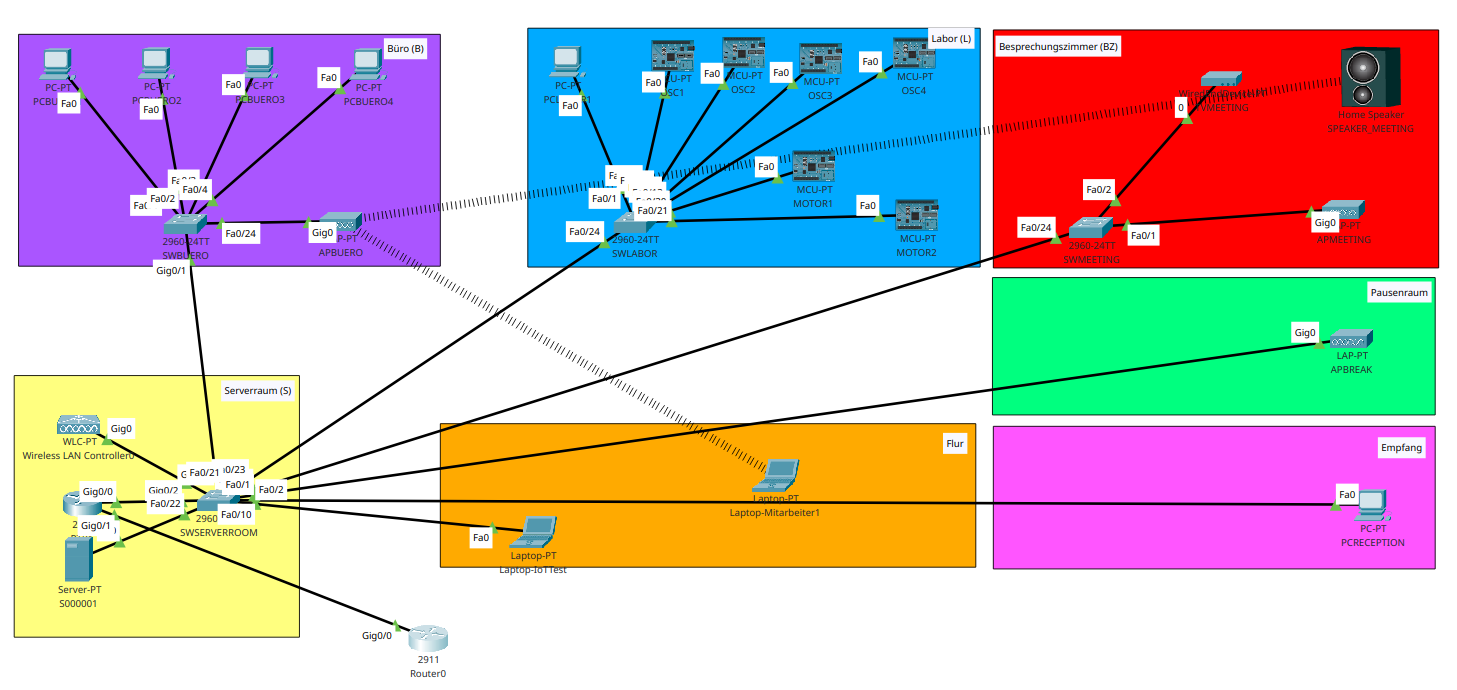
\includegraphics[width=.9\linewidth]{./bfki_projekt_cisco_logical.png}
\end{center}
\section{Dokumentation der ausgeführten Aktionen}
\label{sec:org859bd62}
\subsection{Allgemein}
\label{sec:orgae8e6a0}
\begin{itemize}
\item zuerst die bestehenden Geräte ins Netzwerk aufgenommen
\item für die Oszilloskope und Motorregler Cisco-Gerät ``MCU-PT'' mit 1 FE-Port genommen
\item Zusätzliche Hardware:
\begin{itemize}
\item SWSERVERROOM
\item SWMEETING
\end{itemize}
APBREAK und PCRECEPTION sind via Patch Panel direkt am Hauptswitch SWSERVERROOM angebunden
\item Display Names Prefixes
\begin{itemize}
\item SW Switch
\item RTR Router
\item PC Arbeitsplatz-PC
\item AP Access Point
\item TV Fernseher
\end{itemize}
\item Geräte sind mit dem Raumname SERVERROOM, BUERO, MEETING, LABOR, BREAK, RECEPTION benannt, wenn mehrere gleichartige Geräte in einem Raum vorhanden sind, werden sie ab 1 nummeriert
\item Router wird ohne Raumname benannt und erhält einfach den Namen RTR1
\end{itemize}
\subsection{SWSERVERROOM}
\label{sec:org86be69a}
\begin{itemize}
\item Hostname SWSERVERROOM gesetzt
\begin{verbatim}
hostname SWSERVERROOM
\end{verbatim}
\item logging synchronous für con0 und vty0-4 aktiviert
\begin{verbatim}
line con0
  logging synchronous
line vty 0 4
  logging synchronous
\end{verbatim}
\item VLANs angelegt
\begin{verbatim}
vlan 10
  name "FIRMENNETZ"
vlan 20
  name "IoT-Netz"
vlan 30
  name "Privat-Netzwerk"
vlan 40
  name "WirelessManagement"
vlan 999
  name "Fallback VLAN"
\end{verbatim}
\item Standardkonfiguration für alle Ports erstellen und Ports abschalten
\begin{verbatim}
interface range fa0/1-24,gi0/1-2
  shutdown
  switchport mode access
  switchport access vlan 999
\end{verbatim}
\item Port zu Router (Gi0/2) als Trunk konfiguriert und aktiviert
\begin{verbatim}
interface gi0/2
  description link to RTR1
  switchport mode trunk
  switchport trunk native vlan 999
  switchport trunk allowed vlan 10,20,30,40
  no shutdown
\end{verbatim}
\item Port zu Büro-Switch (Gi0/1) als Trunk konfiguriert und aktiviert
\begin{verbatim}
interface gi0/1
  description link to SWBUERO
  switchport mode trunk
  switchport trunk native vlan 999
  switchport trunk allowed vlan 10,30,40
  no shutdown
\end{verbatim}
\item Port zu SERVER1 (Fa0/22) konfiguriert und aktiviert
\begin{verbatim}
interface fa0/22
  description link to SERVER1
  switchport mode access
  switchport access vlan 10
  no shutdown
\end{verbatim}
\item Port zu Labor-Switch (Fa0/23) als Trunk konfiguriert und aktiviert
\begin{verbatim}
interface fa0/23
  description link to SWLABOR
  switchport mode trunk
  switchport trunk native vlan 999
  switchport trunk allowed vlan 10,20
  no shutdown
\end{verbatim}
\item Port zu Meetingraum-Switch (Fa0/24) als Trunk konfiguriert und aktiviert
\begin{verbatim}
interface fa0/24
  description link to SWMEETING
  switchport mode trunk
  switchport trunk native vlan 999
  switchport trunk allowed vlan 10,30,40
  no shutdown
\end{verbatim}
\item Port zu Pausenraum-Accesspoint (Fa0/1) als Trunk konfiguriert und aktiviert
\begin{verbatim}
interface fa0/1
  description link to APBREAK
  switchport mode trunk
  switchport trunk native vlan 40
  switchport trunk allowed vlan 30,40
  no shutdown
\end{verbatim}
\item Port zu Empfangs-PC (Fa0/2) konfiguriert und aktiviert
\begin{verbatim}
interface fa0/2
  description link to PCRECEPTION
  switchport mode access
  switchport access vlan 10
\end{verbatim}
\item Port zu WLAN-Controller (Fa0/21) konfiguriert und aktiviert
\begin{verbatim}
switchport fa0/21
  description link to Wireless Controller0
  switchport mode access
  switchport access vlan 40
  no shutdown
\end{verbatim}
\end{itemize}
\subsection{SWLABOR}
\label{sec:org58e2240}
\begin{itemize}
\item Hostname SWLABOR gesetzt
\item logging synchronous für con0 und vty0-4 aktiviert
\item VLANs angelegt
\item Alle Switchports Fa0/1-24,Gi0/1-2 shutdown
\item Alle Switchports Fa0/1-24,Gi0/1-2 auf VLAN 999 gesetzt
\item Switchport Fa0/24 (link to SWSERVERROOM) auf Trunk 10,20,30 konfiguriert und up
\begin{verbatim}
interface fa0/24
  description link to SWSERVERROOM
  switchport mode trunk
  switchport trunk native vlan 999
  switchport trunk allowed vlan 10,20,30
  no shutdown
\end{verbatim}
\item Switchport Fa0/1 (link to SWLABOR1) auf Access 10 konfiguriert und up
\begin{verbatim}
interface fa0/1
  description link to SWLABOR1
  switchport mode access
  switchport access 10
  no shutdown
\end{verbatim}
\item Switchports Fa0/10-13 (link to OSCx) auf Access 20 konfiguriert und up
\begin{verbatim}
interface range fa0/10-13
  switchport mode access
  switchport access vlan 20
  no shutdown
\end{verbatim}
\item Switchports Fa0/20-21 (link to MOTORx) auf Access 20 konfiguriert und up
\begin{verbatim}
interface range fa0/20-21
  switchport mode access
  switchport access vlan 20
\end{verbatim}
\end{itemize}
\subsection{SWBUERO}
\label{sec:org775d4b3}
\begin{itemize}
\item Hostname SWBUERO gesetzt
\item logging synchronous für con0 und vty0-4 aktiviert
\item VLANs angelegt
\item Alle switchports Fa0/1-24,Gi0/1-2 shutdown
\item Alle Switchports Fa0/1-24,Gi0/1-2 auf VLAN 999 gesetzt
\item Switchports Fa0/1-4 (link to PCBUEROx) auf access 10 konfiguriert und up
\item Switchport Fa0/24 (link to APBUERO) auf Trunk native VLAN 40, allowed 30 konfiguriert und up
\item Switchport Gi0/1 (link to SWSERVERROOM) auf trunk native 999, allowed 10,30,40 konfiguriert und up
\end{itemize}
\subsection{SWMEETING}
\label{sec:orgdf002a0}
\begin{itemize}
\item Hostname SWMEETING gesetzt
\item logging synchronous fün con0 und vty0-4 aktiviert
\item VLANs angelegt
\item Alle switchports Fa0/1-24,Gi0/1-2 shutdown
\item Alle switchports Fa0/1-24,Gi0/1-2 auf access 999 gesetzt
\item Switchport Fa0/1 (link to APMEETING) auf trunk native VLAN 40, allowed VLANs 30,40 konfiguriert und up
\item Switchport Fa0/24 (link to SWSERVERROOM) auf trunk native 999, allowed 10,30,40 konfiguriert und up
\end{itemize}
\subsection{RTR1}
\label{sec:org4ee8349}
\begin{itemize}
\item Vier Cover in der Physical view hinzugefügt, um die leeren Plätze zu füllen
\item Initialer Assistent übersprungen
\item Hostname RTR1 gesetzt
\item Logging synchronous für line con0 und vty0-15 gesetzt
\begin{verbatim}
line con 0
  logging synchronous
line vty 0 15
  logging synchronous
\end{verbatim}
\item Subinterface Gi0/0.10 mit dot1q 10 konfiguriert und IP-Adresse 172.19.0.1/25, 2001:db8:0:10::1/64, fe80::1 zugewiesen
\begin{verbatim}
interface gi0/0.10
  encapsulation dot1Q 10
  ip address 172.19.0.1 255.255.255.128
  ipv6 address 2001:db8:0:10::1/64
  ipv6 address fe80::1 link-local
\end{verbatim}
\item Subinterface Gi0/0.20 mit dot1q 20 konfiguriert und IP-Adresse 172.19.0.129/25, 2001:db8:0:20::1/64, fe80::1 zugewiesen, helper-adresse zugewiesen
\begin{verbatim}
interface gi0/0.20
  encapsulation dot1Q 20
  ip address 172.19.0.129 255.255.255.128
  ipv6 address 2001:db8:0:20::1/64
  ipv6 address fe80::1 link-local
  ip helper-address 172.19.0.2
\end{verbatim}
\item Subinterface Gi0/0.30 mit dot1q 30 konfiguriert und IP-Adresse 172.19.1.1/25, 2001:db8:0:30::1/64, fe80::1 zugewiesen
\begin{verbatim}
interface gi0/0.30
  encapsulation dot1Q 30
  ip address 172.19.1.1 255.255.255.128
  ipv6 address 2001:db8:0:30::1/64
  ipv6 address fe80::1 link-local
  ip helper-address 172.19.0.2
\end{verbatim}
\item Subinterface Gi0/0.40 mit dot1q 40 konfiguriert und IP-Adresse 172.19.1.129/25, 2001:db8:0:40::1/64, fe80::1 zugewiesen
\begin{verbatim}
interface gi0/0.40
  encapsulation dot1Q 40
  ip address 172.19.1.129 255.255.255.128
  ipv6 address 2001:db8:0:40::1/64
  ipv6 address fe80::1 link-local
  ip helper-address 172.19.0.2
\end{verbatim}
\item Interface Gi0/0 up
\begin{verbatim}
interface gi0/0
  no shutdown
\end{verbatim}
\end{itemize}

Um eine Internetverbindung zu simulieren, haben wir ein weiteres Interface mit einer ``öffentlichen'' IP-Adresse hinzugefügt und den Internetzugriff mit einem NAT den Netzen ermöglicht:

\begin{itemize}
\item Access List für Internetzugriff definieren
\begin{verbatim}
ip access-list standard NAT-SOURCES
  10 permit 172.19.0.0 0.0.0.127
  20 permit 172.19.1.0 0.0.0.127
\end{verbatim}
\item NAT Pool anlegen für Internetzugriff
\begin{verbatim}
ip nat pool ISPGIVEN 45.232.17.12 45.232.17.12 netmask 128.0.0.0
\end{verbatim}
\item Source NAT für Internet definieren und Interface für simulierten Internettraffic erstellen
\begin{verbatim}
ip nat inside source list NAT-SOURCES pool ISPGIVEN
interface gi0/1
  ip address 45.232.17.11 128.0.0.0
  ip nat outside
interface gi0/0.10
  ip nat inside
interface gi0/0.30
  ip nat inside
\end{verbatim}
\end{itemize}

Für die Netzisolation haben wir Access-Lists erstellt und diese den Subinterfaces hinzugefügt:

\begin{verbatim}
ip access-list standard FROMIOT
  10 permit 172.19.0.0 0.0.0.127
  90 deny any

interface gi0/0.20
  ip access-group FROMIOT out


ip access-list standard FROMPRIVAT
  10 deny 172.19.0.0 0.0.0.127
  20 deny 172.19.0.128 0.0.0.127
  30 permit any

interface gi0/0.30
  ip access-group FROMPRIVAT out


ip access-list standard FROMFIRMENNETZ
  10 deny 172.19.1.0 0.0.0.127
  20 permit any

interface gi0/0.10
  ip access-group FROMFIRMENNETZ out
\end{verbatim}
\subsection{SERVER1}
\label{sec:org7e7a06b}
\begin{itemize}
\item Hostname S000001 gesetzt
\item IP-Adressen 172.19.0.2/25, 2001:db8:0:10::2/64 gesetzt
\item DHCP-Server konfiguriert (KONFIG FEHLT)
\item DHCPv6-Server konfiguriert (KONFIG FEHLT)
\item DNS aktiviert ohne Konfig.
\end{itemize}
\subsection{Alle Enddevices (PCx, OSCx, MOTORx, TVx)}
\label{sec:orgdb1535a}
\begin{itemize}
\item Gateway IPv4 und IPv6 via DHCP/automatisch gesetzt
\item FastEthernet0 IPv4 und IPv6 Adressen via DHCP(v6) beziehen
\end{itemize}
\subsection{Wireless LAN Controller}
\label{sec:orgb83ff68}
\begin{itemize}
\item WLAN-Netz Sensoic\_Gast mit VLAN 30, WPA2-PSK Passphrase ``CISCOPacketTracer'', lokale Switching und Authentikation konfiguriert
\item DHCP-Pool aps angelegt mit Gateway 172.19.1.129, DNS 172.19.0.2, Start IP Address 172.19.1.140, Subnetzmask 255.255.255.128, max user 20, WLC address 172.19.1.130
\end{itemize}
\subsection{SPEAKER\_MEETING}
\label{sec:orgc8a8f3a}
\begin{itemize}
\item WLAN-Netzwerk Sensoic\_Gast konfiguriert
\end{itemize}
\subsection{Simuliertes Internet 8.8.8.8}
\label{sec:org814f7fe}

Für die simulierte Internetverbindung haben wir einen weiteren Router mit der IP 8.8.8.8 erstellt und diesen direkt mit unserem Router RTR1 verbunden.

\begin{verbatim}
interface Gi0/0
  ip address 8.8.8.8 128.0.0.0
  no shutdown
\end{verbatim}

Weitere Einstellungen haben wir nicht vorgenommen, da wir diesen Router nur verweden um zu verifizieren, ob Verbindung von den einzelnen Netzen möglich ist.
\subsection{Simuliertes Mitarbeiternotebook}
\label{sec:orge59964c}

Wir haben ein weiteres Notebook ``Laptop-Mitarbeiter1'' hinzugefügt, um Netzwerkrichtlinien für das Privat-Netzwerk zu testen. Dieses wird per WLAN-Verbindung an Sensoic\_Gast angebunden und erhält seine IP-Adresse per DHCP.
\subsubsection{Tests}
\label{sec:orgd481ba7}
\begin{itemize}
\item[{$\boxtimes$}] VLAN 30 kann ins Internet sprechen [getestet als Ping an 8.8.8.8]
\item[{$\boxtimes$}] VLAN 30 kann nicht in das Firmennetz sprechen [getestet als Ping an 172.19.0.103]
\item[{$\boxtimes$}] VLAN 30 kann nicht in das IoT-Netz sprechen [getestet als Ping an 172.19.0.146]
\end{itemize}
\subsection{Simuliertes Notebook im VLAN 20 (IoT-Netz)}
\label{sec:org46c6356}

Wir haben ein weiteres Notebook ``Laptop-IoTTest'' hinzugefügt, um Netzwerkrichtlinien für das IoT-Netzwerk zu testen. Dieses wird per LAN direkt am SWSERVERROOM angebunden (Fa0/10) und erhält seine IP-Adresse per DHCP.
\subsubsection{Tests}
\label{sec:orgfd27967}

\begin{itemize}
\item[{$\boxtimes$}] VLAN 20 kann nicht ins Internet (NAT-Zugang über Access-List NAT-SOURCES blockiert) [getestet als Ping an 8.8.8.8]
\item[{$\boxtimes$}] VLAN 20 kann in das Firmennetzwerk sprechen [getestet als Ping an 172.19.0.103 (PCBUERO1)]
\item[{$\boxtimes$}] VLAN 20 kann nicht in das Privatnetzwerk sprechen [getestet als Ping an 172.19.1.16 (Laptop-Mitarbeiter1)]
\end{itemize}
\end{document}
